\documentclass[11pt]{article}

\usepackage{apacite}
\usepackage{amsmath,amssymb}
\usepackage{graphicx}
\usepackage{color}
\usepackage{url}
\usepackage{fullpage}
\usepackage{setspace}
\usepackage{booktabs}
\usepackage{multirow}
\usepackage{lingmacros}
\usepackage{caption}
\usepackage{subcaption}

%\newcommand{\url}[1]{$#1$}

\definecolor{Blue}{RGB}{50,50,200}
\newcommand{\blue}[1]{\textcolor{Blue}{#1}}

\definecolor{Red}{RGB}{255,0,0}
\newcommand{\red}[1]{\textcolor{Red}{#1}}
\newcommand{\jd}[1]{\textcolor{Red}{[jd: #1]}} 

\definecolor{Green}{RGB}{50,200,50}
\newcommand{\ndg}[1]{\textcolor{Green}{[ndg: #1]}}  

 \newcommand{\denote}[1]{\mbox{ $[\![ #1 ]\!]$}}


\newcommand{\subsubsubsection}[1]{{\em #1}}
\newcommand{\eref}[1]{(\ref{#1})}
\newcommand{\tableref}[1]{Table \ref{#1}}
\newcommand{\figref}[1]{Figure \ref{#1}}
\newcommand{\appref}[1]{Appendix \ref{#1}}
\newcommand{\sectionref}[1]{Section \ref{#1}}


\title{Over overinformativeness: rational redundant referring expressions}

 
\author{{\large \bf Judith Degen, Caroline Graf, Robert X.D.~Hawkins, Noah D.~Goodman} \\
  \{jdegen,ngoodman\}@stanford.edu\\
  Department of Psychology, 450 Serra Mall \\
  Stanford, CA 94305 USA}

\begin{document}

\maketitle


\begin{abstract}
 

\textbf{Keywords:} 
reference; referring expressions; informativeness; probabilistic pragmatics; experimental pragmatics
\end{abstract}

\section{Introduction}
\label{sec:intro}

Reference to objects is one of the most basic and prevalent uses of language. But how do speakers choose amongst the wealth of referring expressions they have at their disposal? How does a speaker choose whether to refer to an object as \emph{the animal}, \emph{the dog}, \emph{the dalmatian}, or \emph{the big mostly white dalmatian}? The context within which the object occurs  (other non-dogs, other dogs, other dalmatians) plays a large part in determining which features the speaker chooses to include in their utterance  -- speakers aim to be sufficiently informative to uniquely establish reference to the intended object. However, speakers' utterances often exhibit what has been claimed to be \emph{overinformativeness}: referring expressions are often more specific than necessary for establishing unique reference, and they are so in systematic ways. However, providing a unified theory for speakers' systematic patterns of overinformativeness has so far proved elusive.

This paper is concerned with  modeling precisely this choice of referring expression (RE). We restrict ourselves to definite descriptions of the form \emph{the (ADJ}?\emph{)}+ \emph{NOUN}, that is, noun phrases that minimally contain the definite determiner \emph{the} followed by a head noun. In addition, any number of adjectives may occur between the determiner and the noun.\footnote{In contrast, we will \emph{not} provide a treatment of pronominal referring expressions, indefinite descriptions, names, or definite descriptions with post-nominal modification, though we offer some speculative remarks on how the approach outlined here can be applied to these cases. \jd{make sure you actually do this in the gd.}} A model of these REs will allow us to unify two domains in language production that have been typically treated as separate, and that have typically been treated as interesting for different reasons: the production of so-called overmodified referring expressions on the one hand, which a lot of literature in language production has been devoted to \cite{deutsch, hermann, Pechmann1989, nadig2002,  Maes2004, Engelhardt2006, Arts2011, Koolen2011, rubiofernandez2016}; and the production of simple nominal expressions, which has so far mostly received attention in the concepts and categorization literature \cite{bla bla}. In the following, we review some of the key phenomena and puzzles in each of these literatures which have for the most part been treated as unrelated. We then present a model of RE production within the Rational Speech Acts \cite{frank2012} framework, which treats speakers as boundedly rational agents that try to optimize the tradeoff between utterance cost and  informativeness. Our key innovation is to relax the assumption that semantic truth functions are deterministic. \jd{one sentence here that inspires intuition, or a paragraph foreshadowing, making it seem like the obvious solution?} It is this crucial innovation that allows us to provide a unified explanation for a great number of seemingly disparate phenomena from the modified and nominal RE literature.

\subsection{Production of referring expressions: a case against rational language use?}

How should a cooperative speaker produce referring expressions? Grice, in his seminal work, provided some guidance by formulating his famous conversational maxims, intended as a guide to listeners' expectations about good speaker behavior \cite{grice1975}. His maxim of Quantity, consisting of two parts, requires of speakers to:

\begin{enumerate}
	\item \emph{Quantity-1:} Make your contribution as informative as s required (for the purposes of the exchange).
	\item \emph{Quantity-2:} Do not make your contribution more informative than is required.
\end{enumerate}

That is, speakers should aim to produce neither under- nor overinformative utterances. While much support has been found for the former \cite{lots of people}, speakers seem remarkably happy to systematically violate Quantity-2. In modified referring expressions, they routinely produce modifiers that do not uniquely establish reference (e.g., \emph{the small blue thumbtack} instead of \emph{the small thumbtack} in contexts like \figref{fig:sizesufficient} \cite{bla bla}). In simple nominal expressions, speakers routinely choose to refer to an object with a basic level term even when a superordinate level term would have been sufficient for establishing reference (e.g., \emph{the dog} instead of \emph{the animal} in contexts like \figref{fig:dogcontexts}d \cite{bla bla}).

These observations have posed a challenge for theories of language production, especially those positing rational language use (including the Gricean one): why this extra expenditure of useless effort? Why this seeming blindness to the level of informativeness requirement? Many have argued from these observations that speakers are in fact not economical \cite{bla}. Some have derived a built-in preference for referring at the basic level from considerations of \jd{bla} and \jd{bla} \cite{Rosch1976}. Others have argued for salience-driven effects on willingness to overmodify \cite{dutch guys}. In all cases, it is argued that informativeness cannot be the key factor in determining the content of speakers' referring expressions.

Here we revisit this claim and show that systematically relaxing the requirement of a deterministic semantics for referring expressions also systematically changes the informativeness of utterances. This results in a reconceptualization of what have been termed \emph{overinformative referring expressions} as \emph{rationally redundant referring expressions}. We begin by reviewing the phenomena of interest that a revised theory of definite referring expressions should be able to account for. 

\subsection{Modified referring expressions}
\label{sec:modified}


Most of the literature on overinformative referring expressions has been devoted to the use of overinformative modifiers in modified referring expressions. The prevalent observation is that speakers frequently do not include only the minimal modifiers required for establishing unique reference, but often also include redundant modifiers \cite{Pechmann1989, nadig2002,  Maes2004, Engelhardt2006, Arts2011, Koolen2011}. However, not all modifiers are created equal: there are systematic differences in the overmodification patterns observed for size adjectives (e.g., \emph{big, small}), color adjectives (e.g., \emph{blue, red}), material adjectives (e.g., \emph{plastic, wooden}), and many others. Here we review some of the intriguing patterns of overmodification that have plagued that literature, focusing for the most part on size and color.



\begin{figure}
\begin{subfigure}{.5\textwidth}
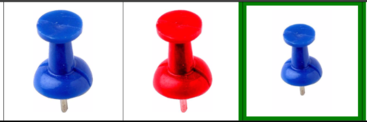
\includegraphics[width=\textwidth]{pics/size-sufficient.png}
\caption{Size sufficient.}
\label{fig:sizesufficient}
\end{subfigure}
\begin{subfigure}{.5\textwidth}
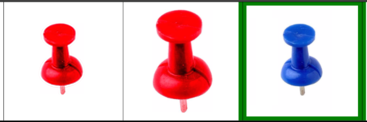
\includegraphics[width=\textwidth]{pics/color-sufficient.png}
\caption{Color sufficient.}
\label{fig:colorsufficient}
\end{subfigure}
\caption{Example contexts where size vs.~color is sufficient for unique reference. A green border marks the intended referent.}
\label{fig:thumbtack}
\end{figure}

\begin{figure}
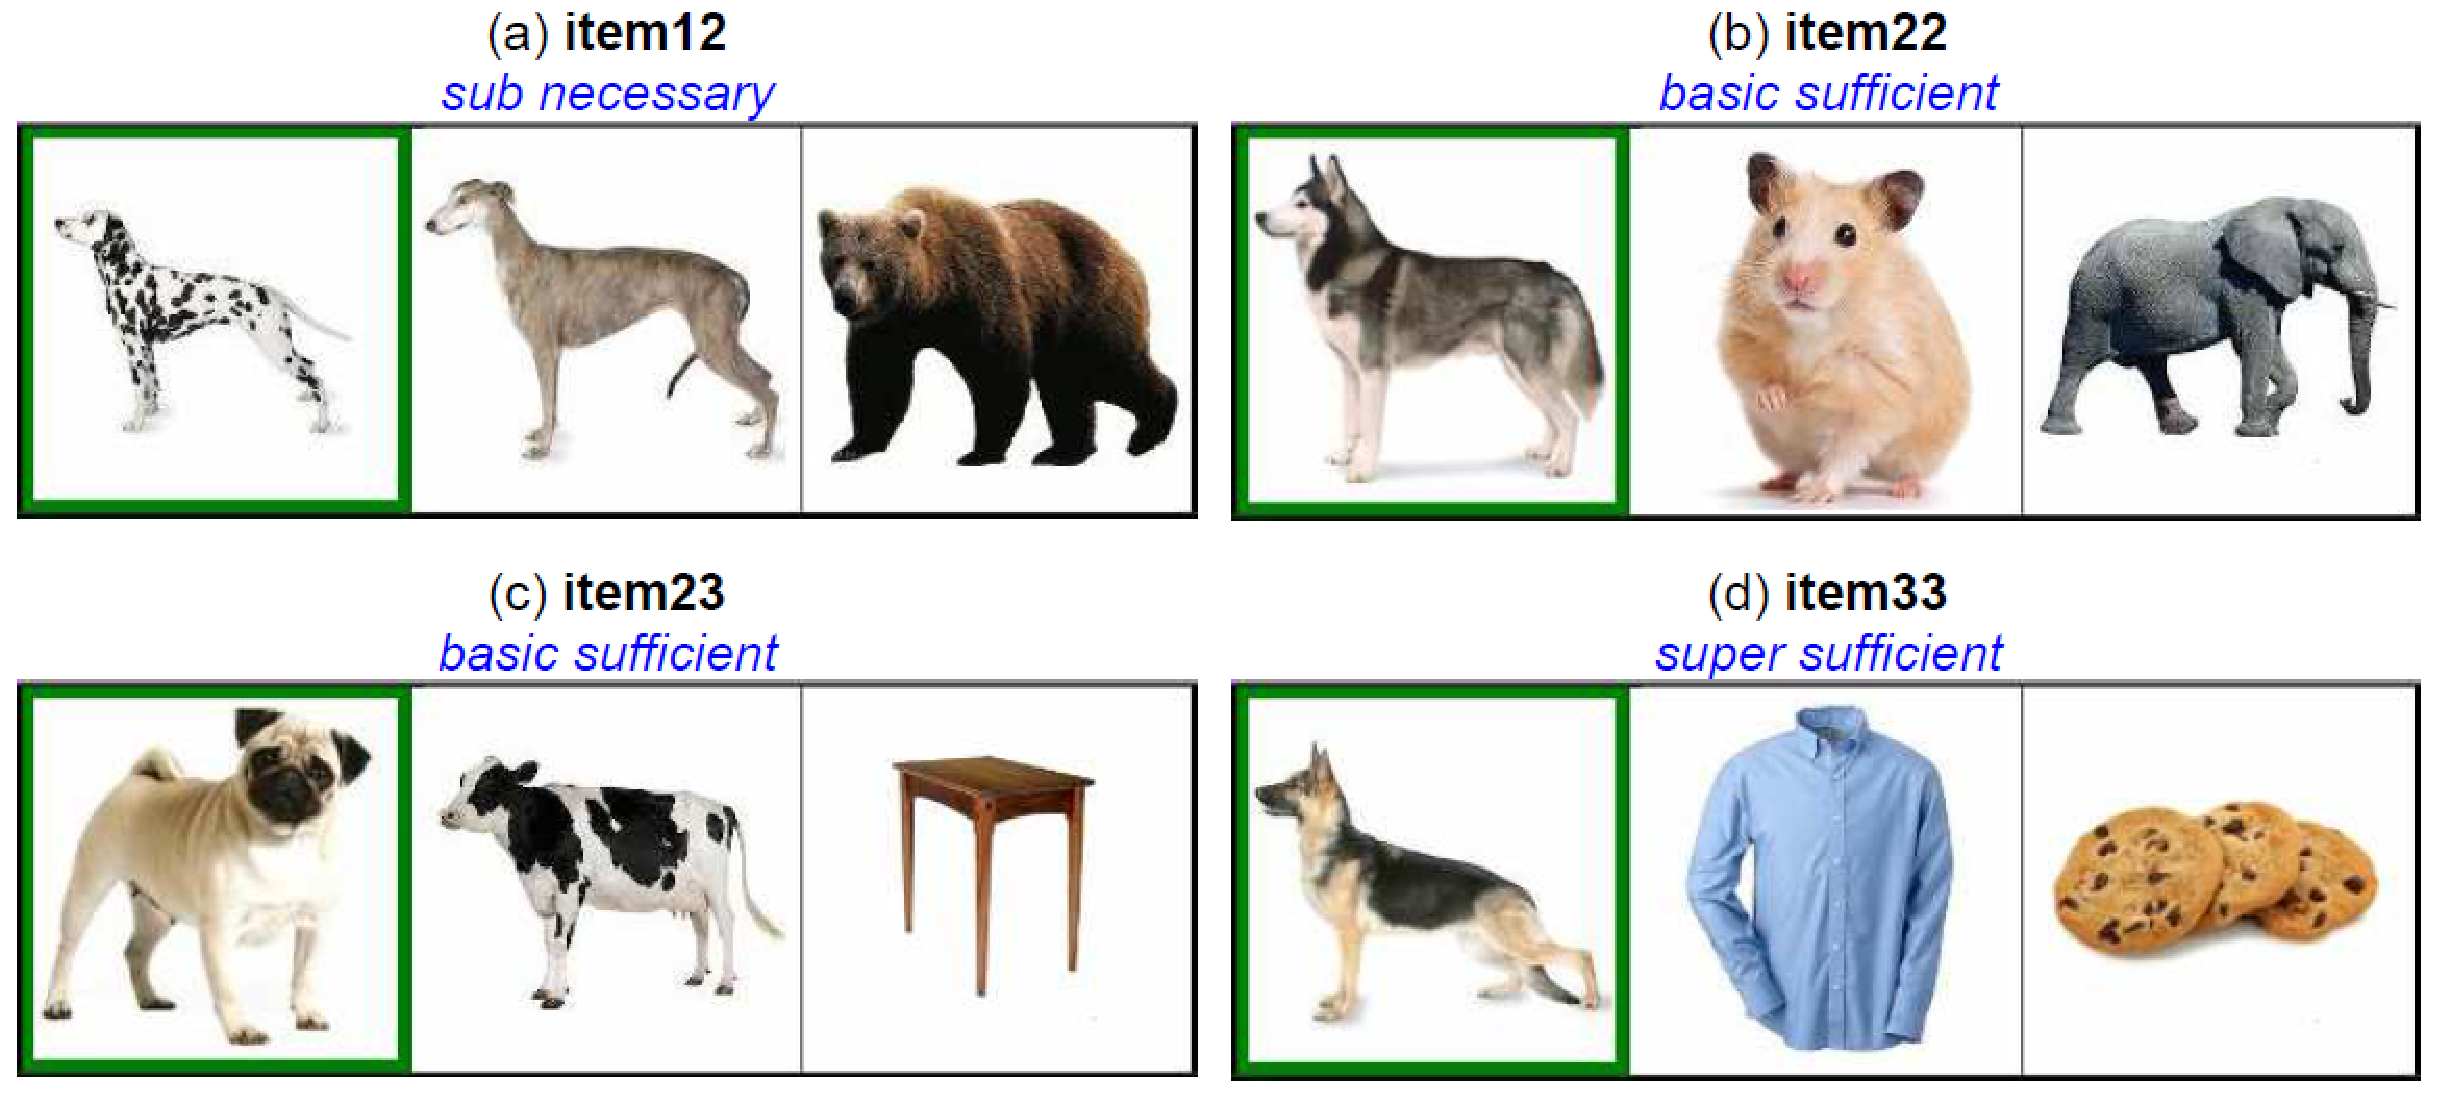
\includegraphics[width=\textwidth]{pics/design}
\caption{Example contexts where at least the sub (\emph{dalmatian}, a), basic (\emph{dog}, b, c), or the super (\emph{animl}, d) level term are necessary for establishing unique reference. A green border marks the intended referent.}
\label{fig:dogcontexts}
\end{figure}

\subsubsection{Asymmetry in redundant use of color and size adjectives}
\label{sec:asymmetry}

 In \figref{fig:sizesufficient}, singling out the object with the green border requires only mentioning its size, as in \emph{the small thumbtack}. But it is now well-documented that speakers routinely include redundant color adjectives as in \emph{the small blue thumbtack}, which do not uniquely single out the intended referent in these kinds of contexts \cite{Pechmann1989,  Belke2002, gatt2011}. However, the same is not true for size: in contexts like \figref{fig:colorsufficient}, where color is sufficient for unique reference (\emph{the blue thumbtack}), speakers overmodify much more rarely with size. \tableref{tab:colorsizeasymmetry} shows proportions of color, size, and (overinformative) color-and-size mentions in conditions like those depicted in \figref{fig:thumbtack} across different experiments. In all cases there is a preference for overmodifying with color but not with size.\footnote{There is quite a bit of variation in the actual numbers. We will discuss this variation in the General Discussion. \jd{or already in the model section where we get the basic asymmetry}}
 
 \begin{table}
 \caption{Proportions of minimally informative \emph{color} or \emph{size} and overinformative \emph{color\_size} mentions in color-sufficient vs.~size-sufficient conditions across experiments.\jd{keep filling in.}}
 	\begin{tabular}{l l l l l l l l}
	\toprule
	 & & \multicolumn{3}{c}{Color sufficient} & \multicolumn{3}{c}{Size sufficient} \\
	Study & Language & \emph{color} & \emph{size} & \emph{color\_size}  & \emph{color} & \emph{size} & \emph{color\_size} \\
	\midrule
	\citeA{Pechmann1989} & Dutch & 99 & 0 & 1 & 9 & 36 & 55 \\
	\citeA{gatt2011} & English & 92 & 0 & 8 & 3 & 17 & 80\\
 	\citeA{gatt2011} & Dutch & 90 & 0 & 10 & 0 & 21 & 79 \\	
 Our baseline study & English & 94 & 0 & 6 & 2 & 52 & 46 \\ 
	\bottomrule
	\end{tabular}
	\label{tab:colorsizeasymmetry}
 \end{table}

Explanations for this asymmetry have varied. \citeA{Pechmann1989} was the first to take the asymmetry as evidence for speakers following an incremental strategy of object naming: speakers initially start to articulate an adjective denoting a feature that listeners can quickly and easily recognize (i.e., color) before they have fully inspected the display and extracted the sufficient dimension. However, this would predict that speakers routinely should produce expressions like \emph{the blue small thumbtack}, which violate the preference for size adjectives to occur before color adjectives in English \cite{bla adjective ordering prefs}. While Pechmann did observe such violations in his dataset, most cases of overmodification did not constitute such violations, and he himself concludes that incrementality cannot (on its own) account for the asymmetry in speakers' propensity for overmodifying with color vs.~size.  


Another explanation for the asymmetry is that speakers try to produce modifiers that denote features that are reasonably easy for the listener to perceive, so that, even when a feature is not fully distinguishing in context, it at least serves to restrict the number of objects that could plausibly be considered the target. Indeed, there has been some support for the idea that overmodification can be beneficial to listeners by facilitating target identification \cite{arts2011, rubiofernandez2016}.

\jd{try to find a quote from someone who says it's all just a matter of cost?}

There have been various attempts to capture the color-size asymmetry in computational natural language generation models. The earliest contenders for models of definite referring expressions like the Full Brevity algorithm \cite{Dale1989} or the Greedy algorithm \cite{Dale1989} focused only on discriminatory value -- that is, an utterance's informativeness -- in generating referring expressions, which resulted in an inability to capture the color-size asymmetry: the models only produced the minimally specified expressions. Subsequently, the Incremental algorithm \cite{dale1995} incorporated a preference order on features, with color ranked higher than size. The order is traversed and each encountered feature included in the expression if it serves to exclude at least one further distractor. This results in the production of overinformative color but not size adjectives. However, the resulting asymmetry is much greater than that evident in human speakers, and is deterministic rather than exhibiting the probabilistic production patterns that human speakers exhibit. More recently, the PRO model \cite{GattEtAl2013} has sought to integrate the observation that speakers seem to have a preference for including color terms with the observation that a preference does not imply the deterministic inclusion of said color term. The model is specifically designed to capture the color-size asymmetry: in a first step, the uniquely distinguishing property (if there is one) is first selected deterministically.  In a second step, an additional property is added probabilistically, depending on both a salience parameter associated with the additional property and a parameter capturing speakers' eagerness to overmodify. If both properties are uniquely distinguishing, a property is selected probabilistically depending on its associated salience parameter. The second step proceeds as before.

However, while the PRO model -- the most state-of-the-art computational model of human production of modified referring expressions -- can capture the color-size asymmetry in and of itself, it is neither flexible enough to be extended straightforwardly to other modifiers beyond color and size, nor can it straightforwardly be extended to capture the more subtle systematicity with which the preference to overmodify with color changes based on various features of context. We delve into these more subtle patterns in the next two sections before presenting our alternative model within the Rational Speech Acts framework.

\subsubsection{Scene variation}
\label{sec:scenevariation}

Speakers' propensity to overmodify with color is highly dependent on features of the distractor objects in the context. In particular, as the variation present in the scene increases, so does the probability of overmodifying with color \cite{Davies2013, Koolen2013}. How exactly scene variation is quantified differs between papers. One very clear demonstration of the scene variation effect was given by \citeA{Koolen2013}, who quantified scene variation as the number of feature dimensions along which objects in a scene vary. Over the course of three experiments, they compared a low-variation condition in which objects never differed in color with a high-variation condition in which objects differed in type, color, orientation, and size. They consistently found higher rates of overmodification with color in the high-variation (28-27\%) than in the low-variation (4-10\%) conditions.

The effect of scene variation on propensity to overmodify has typically been explained as the result of the demands imposed on visual search: in low-variation scenes, it is easier to discern the discriminating dimensions than in high-variation scenes, where it may be easier to simply start naming features of the target that are salient \cite{Koolen2013}. 

The PRO model does not have a straightforward way of capturing the effect of scene variation on probability of overmodification. One way of doing so is to make the salience and overmodification parameters directly dependent on the amount of variation in the scene. However, this requires additional free parameters and makes the model prone to overfitting. \jd{elaborate or clean up}

\subsubsection{Feature typicality}
\label{sec:colortypicality}


Overmodification with color has been shown to be systematically related to the typicality of the color for the object. Building on work by \citeA{sedivy2003a}, \citeA{Westerbeek2015} (and more recently, \citeA{rubiofernandez2016}) have shown that the more typical a color is for an object, the less likely it is to be mentioned when not necessary for unique reference. For example, speakers never refer to a yellow banana as \emph{the yellow banana}, but they sometimes refer to a brown banana as \emph{the brown banana}, and they almost always refer to a blue banana as \emph{the blue banana}. In fact, color typicality and probability exhibit a linear negative correlation \cite{Westerbeek2015}. Similar typicality effects have been shown for other (non-color) properties. For example, \citeA{Mitchell2013} showed that speakers are more likely to include an atypical than a typical property (either shape or material) when referring to everyday objects like boxes when mentioning at least one property was necessary for unique reference. %, when the shape and material was atypical (e.g., heart-shaped, made of clay) than when it was typical (e.g., square, made of cardboard). 

Whether speakers are more likely to mention atypical properties over typical properties because they are more salient to \emph{them} or because they are trying to make reference resolution easier for the listener, for whom presumably these properties are also salient, is an open question \cite{Westerbeek2015}. Some support for the audience design account comes from a study by \citeA{Huettig2011}, who found that listeners, after hearing a noun with a diagnostic color (e.g., \emph{frog}), are more likely to fixate objects of that diagnostic color (green), indicating that typical object features are rapidly activated and aid visual search. Nevertheless, the benefit for listeners and the salience for speakers might simply be a happy coincidence and speakers might not, in fact, be designing their utterances for their addressees. We will remain agnostic about the underlying reason for typicality effects \jd{will we, though? the model assumes that typicality affects the literal listener, who speakers reason about, so in a sense we're making a strong audience design claim.}

Irrespective of the source of typicality effects, it is unclear how the PRO model could accommodate them. As for the scene variation effects, it is possible to make the salience and overmodification eagerness parameters directly dependent on the typicality of the feature value for the object the speaker wants to refer to. However, as mentioned above, in the absence of a principled motivation for the way in which these parameters interact, this is simply an exercise in model-fitting without adding explanatory value. In addition, one is left with the task of explaining how scene variation and typicality should interact. 

\subsection{Nominal referring expressions}
\label{sec:nominal}

A problem related to the issue of how many additional features to include in a modified referring expression, but which has received much less attention in the language production literature, is that of deciding at which taxonomic level to refer to an object to in a simple nominal expression. That is, even in the absence of adjectives, a referring expression can be more or less informative: \emph{the dalmatian} communicates more information about the object in question than \emph{the dog}, which in turn is globally more informative than \emph{the animal}. Thus, this choice can be considered analogous to the choice of adding more modifiers -- in both cases, the speaker has a choice of being more or less specific about the intended referent. However, the choice of reference level in simple nominal referring expressions is also interestingly different from that of adding modifiers in that there is no additional word-level cost associated with being more specific -- the choice is between different one-word utterances, not between utterances of different lengths (in words). 

Nevertheless, cost affects the choice of reference level: in particular, speakers prefer more frequent nouns over less frequent ones \cite{bla}, and they prefer shorter ones over longer ones \cite{bla}. This may go part of the way towards explaining the well-documented effect from the concepts and categorization literature that speakers prefer to refer at the \emph{basic level} \cite{Rosch1976}. That is, in the absence of other constraints, even when a superordinate level term would be sufficient for establishing reference (as in \figref{fig:dogcontexts}d), speakers prefer to say \emph{the dog} rather than \emph{the animal}. However, there are nevertheless cases  of contexts where either the superordinate (\figref{fig:dogcontexts}d) or the basic level (\figref{fig:dogcontexts}b and \figref{fig:dogcontexts}c) term would be sufficient for unique reference, where speakers prefer to use the subordinate level term \emph{the dalmatian} \cite{someone who discusses typicality?}.



\jd{Still not entirely sure what all to discuss here. The generally rich interplay between informativeness, cost, and typicality? Or just focus on the basic level preference?}

\subsection{Summary}
\label{sec:introsummary}

In sum, the production of modified and simple nominal referring expressions is governed by a rich interplay of many factors, including an utterance's informativeness, its cost relative to alternative utterances, and the typicality of an object or its features. We are here especially interested in cases where speakers appear to be overinformative -- either by adding more modifiers or by referring at a more specific level than necessary for establishing unique reference. A summary of the effects we will focus on in the remainder of the paper is provided in \tableref{tab:effects}.

\begin{table}
\caption{List of effects a theory of referring expression production should account for.}
\begin{tabular}{l p{6cm} p{5.5cm} }
\toprule
Effect & Description & Reported by \\
\midrule
Color/size asymmetry & More redundant use of color adjectives than size adjectives &  \citeA{Pechmann1989, Engelhardt2006, gatt2011} \red{others}\\
%Number of distractors & More redundant use of color with increasing number of distractors & ?? \red{deutsch} \\
Scene variation & More redundant use of color adjectives with increasing scene variation & \citeA{davies2009, Koolen2013}\\
Color typicality & More redundant use of color adjectives with decreasing color typicality & \citeA{sedivy2003a, Westerbeek2015, rubiofernandez2016}\\
\midrule
Basic level preference & Preference for basic level term when superordinate level term sufficient & \citeA{Rosch1976} \red{others}\\
Subordinate level mention & Unnecessary use of sub level term when basic or super level sufficient & \red{who?}\\
\red{other??} \\
\bottomrule
\end{tabular}
\label{tab:effects}
\end{table}


To date, there is no theory to account for all of these different phenomena; and no model has attempted to unify overinformativeness in the domain of modified and nominal referring expressions. We touched on some of the explanations that have been proposed for these phenomena. We also highlighted where computational models have been proposed for individual phenomena, and how they fall short. In the next section, we present the Rational Speech Acts modeling framework, within which we will provide precisely the kind of theory that can account for at least all of the phenomena listed here and holds great promise for scaling up to many other overinformativeness phenomena.  


\section{Modeling speakers' choice of referring expression}
\label{sec:models}

Here we propose an extension to the production component of the Rational Speech Acts \cite<RSA>{frank2012, goodmanstuhlmueller2013} modeling framework. This extension provides a principled explanation for the phenomena reviewed in the previous section and  holds promise for being generalizable to many further production phenomena related to overinformativeness, which we discuss in the General Discussion. \jd{make a list and make sure to discuss} We proceed by first presenting the general framework in \sectionref{sec:basicrsa}, and show why the most basic model cannot account for any of the phenomena outlined above, due to its strong focus on maximizing the informativeness of one-word expressions under a deterministic semantics. In \sectionref{sec:modifiedmodel} we introduce the crucial innovation: relaxing the assumption of a deterministic semantics. We show that the model can qualitatively account both for speakers' asymmetric propensity to overmodify with color rather than with size and for speakers' propensity to overmodify more with increasing scene variation. In \sectionref{sec:exp1-scenevar} we report an interactive  reference game experiment which functions as a quantitative test of the model. In \sectionref{sec:reflevelmodel} we apply the model to the choice of simple nominal referring expressions and show that the qualitative preference for referring at the basic level emerges from the interaction of informativeness, utterance cost, and typicality. In \sectionref{sec:exp2-reflevel} we then report a second interactive reference game experiment that provides data for a quantitative test of the model. For both cases -- modified and unmodified referring expressions -- we find that a systematic softening of the semantic truth functions results in excellent quantitative fits to the data.


\jd{Interesting snippet from Pechmann which we should probably quote: ``in information theory, a positive function is assigned to redundancy, since it can compensate for partial loss of information. Can overspecification in referential communication have the same function? We can rule out this possibility, because we regard those utterances as being `redundant' which include nondistinguishing features in addition to distinguishing ones. Yet nondistinguishing features cannot compensate for the loss of distinguishing information, since by definition nondistinguishing features do not distinguish the target referent from context. At best, they can reduce the domain of referential alternatives.'' $\rightarrow$ But that IS compensating!}

\subsection{Basic RSA}
\label{sec:basicrsa}

As has been pointed out by \citeA{GattEtAl2013}, the basic Rational Speech Acts model as formulated by \citeA{frank2012} cannot generate overinformative referring expressions for two reasons: first, it trivially cannot do so because it is limited to one-word utterances \cite<see also>{baumann2014}. But even when allowing two-word (or $n$-word) utterances, the speaker's utility will never allow for producing more redundant than minimal referring expressions as long as words contribute non-negative costs to the overall utterance cost. To see this, and as a basis for the innovations introduced in \sectionref{sec:modifiedmodel} and \sectionref{sec:reflevelmodel} it is useful to reiterate the basic form of the model.

Intuitively, the production component of RSA aims to soft-maximize the utility of utterances, where utility is defined in terms of the contextual informativeness of an utterance, given each utterance's literal semantics. Formally, this is treated as a pragmatic speaker $S_1$ reasoning about a literal listener $L_0$, who can be described by the following formula:

\begin{equation}
P_{L_0}(o | u) \propto \denote{u}(o).
\end{equation}

The literal listener $L_0$ hears an utterance $u$ from the set of available one-word utterances $U$ in the context of a set of objects  $O$ and forms a distribution over the referenced object, $o \in O$. Here, $\denote{u}(o)$ is the deterministic lexical meaning of the utterance $u$ when applied to object $o$. That is, $P_{L_0}(o | u)$ returns a uniform distribution over all $o$ denoted by $u$. For example, in the context shown in \figref{fig:sizesufficient}, $U = \{\textrm{\emph{big}}, \textrm{\emph{small}}, \textrm{\emph{blue}}, \textrm{\emph{red}}\}$ and $O = \{o_{\textrm{big\_blue}}, o_{\textrm{big\_red}}, o_{\textrm{small\_blue}}\}$. The values of $P_{L_0}(o | u)$ for each $u$ are shown on the left in \tableref{tab:detliteral}.

\begin{table}
%\centering
\caption{Literal listener distributions $P_{L_0}(o | u)$ for each utterance $u$ in the context depicted in \figref{fig:sizesufficient}, allowing only one-word utterances (left) or one- and two-word utterances (right).}
\begin{tabular}{l r r r}
\toprule
& $o_{\textrm{big\_blue}}$ & $o_{\textrm{big\_red}}$ & $o_{\textrm{small\_blue}}$ \\
\midrule
\emph{big} & .5 & .5 & 0\\
\emph{small} & 0 & 0 & 1\\
\emph{blue} & .5 & 0 & .5\\
\emph{red} & 0 & 1 & 0\\
\bottomrule
\end{tabular}
\begin{tabular}{l r r r}
\toprule
& $o_{\textrm{big\_blue}}$ & $o_{\textrm{big\_red}}$ & $o_{\textrm{small\_blue}}$ \\
\midrule
\emph{big} & .5 & .5 & 0\\
\emph{small} & 0 & 0 & 1\\
\emph{blue} & .5 & 0 & .5\\
\emph{red} & 0 & 1 & 0\\
\emph{big blue} & 1 & 0 & 0\\
\emph{big red} & 0 & 1 & 0\\
\emph{small blue} & 0 & 0 & 1\\
\bottomrule
\end{tabular}
\label{tab:detliteral}
\end{table}

The pragmatic speaker in turn produces an utterance proportional to the utility of that utterance, where utility is a function of both the utterance's \emph{informativeness}  with respect to the literal listener $\ln P_{L_0}(o | u)$ and the utterance's \emph{cost} $c(u)$:

\begin{equation}
P_{S_1}(u | o) \propto e^{\lambda \ln P_{L_0}(o | u) - \beta_c c(u)}
\end{equation}

Both the informativeness and the cost term receive a weight.\footnote{In fact, \citeA{frank2012} did not include a cost weight in their formulation and since they ultimately assumed equal costs for all utterances, they made no use of the cost function. Subsequent work has shown that taking into account utterance cost is necessary for modeling certain interpretation phenomena like cost-based quantity implicatures \cite{degenfrankejaeger2013} and M-implicature \cite{bergen2015}. The cost function will become important for our purposes in a little while.}   Informativeness is weighted by $\lambda$. To understand the effect of $\lambda$, assume that costs are equal and the cost function can thus be disregarded. As $\lambda$ approaches infinity, the speaker increasingly only chooses utterances that maximize informativeness; if $\lambda$ is 0, informativeness is disregarded and the speaker chooses randomly from the set of all available utterances; if $\lambda$ is 1, the speaker probability-matches. For our example in \tableref{tab:detliteral}, if the speaker wants to refer to $o_{\textrm{small\_blue}}$ she has two semantically possible utterances, \emph{small} and \emph{blue}, where \emph{small} is twice as informative as \emph{blue}. She will produce \emph{small} with the following probabilities as $\lambda$ varies: $P_{S_1}(\textrm{\emph{small}} | o_{\textrm{small\_blue}} ; \lambda = \infty) = 1$, $P_{S_1}(\textrm{\emph{small}} | o_{\textrm{small\_blue}} ; \lambda = 1) = \frac{2}{3}$, $P_{S_1}(\textrm{\emph{small}} | o_{\textrm{small\_blue}} ; \lambda = 0) = \frac{1}{4}$. Similarly, if we ignore informativeness and focus only on costs, any asymmetry in costs will be exaggerated with increasing $\beta_c$, such that the speaker will choose the least costly utterance with higher and higher probability as $\beta_c$ increases.

As noted above, this model cannot generate redundant referring expressions for multiple reasons. One of these is trivial: $U$ only contains one-word utterances. We can ameliorate this easily by allowing complex two-word utterances. We assume an intersective semantics for complex utterances $u_{\textrm{complex}}$ consisting of two sub-utterances $u_{\textrm{size}} \in \{\textrm{\emph{big}}, \textrm{\emph{small}}\}$ and $u_{\textrm{color}} \in \{\textrm{\emph{blue}}, \textrm{\emph{red}}\}$, such that $\denote{u_{\textrm{complex}}} = \denote{u_{\textrm{size}}} \wedge\denote{u_{\textrm{color}}}$. The resulting literal listener distributions are shown on the right in \tableref{tab:detliteral}. 

Does this now allow for generating redundant referring expressions? To answer this, let's turn again to the case where the speaker wants to communicate the small blue object. There are now two  utterances, \emph{small} and \emph{small blue}, which are both more informative than \emph{blue} and equally informative to each other, for referring to the small blue object. Because they are equally informative in context, what we need is for the complex utterance to be the \emph{cheaper} one in order to tilt the scales in its favor. While this achieves the desired effect mathematically, the cognitive plausibility of complex utterances being cheaper than simple utterances is highly dubious. But this is the only circumstance under which overinformative referring expressions will be produced with a greater probability than minimally specified referring expressions. Thus, unless we want to introduce a highly dubious cost assumption into the model, we must look elsewhere to account for overinformativeness: to the computation of informativeness itself. This is what we turn to next.

\subsection{RSA with non-deterministic semantics}
\label{sec:modifiedmodel}

\red{you probably should give the intuition for why the fidelity asymmetry should go in the direction that it does BEFORE talking about the plot}

Here we introduce the crucial innovation: rather than assuming a deterministic truth-conditional semantics that returns 1 (true) or 0 (false) for any combination of expression and object, we assume a non-deterministic semantics that can return intermediate values. That is, rather than assuming that an object is unambiguously big or unambiguously blue, we allow for a non-deterministic semantics, capturing that objects count as big or blue to  varying degrees. In particular, consider some of the notable differences between color and size adjectives: color adjectives are considered to fall in the class of absolute adjectives while size adjectives are inherently relative \cite{kennedymcnally2005} -- that is, size adjectives are vague and context-dependent in a way that color adjectives are not. In addition, color as a property has been claimed to be inherently salient in a way that size is not \cite{arts2011,gattetal2013}. Finally, we have shown in recent work that color adjectives are much less subjective in their interpretation than size adjectives \cite{scontrasunderreview}. We use these observations as motivation for exploring the effects of the assumption that the semantics of size adjectives is inherently noisier than the semantics of color adjectives.


Formally, $\denote{u}(o) = exp(\textrm{fidelity}(u,o))$, where $\textrm{fidelity(u,o)}$ returns a number between 0 and 1. The higher an utterance type's fidelity, the less noisy it is and the more likely it is to correctly pick out objects with the denoted property. The lower an utterance type's fidelity, the noisier it is and the more likely it is to incorrectly pick out objects that don't exhibit the denoted property. \red{this isn't quite right}

The effects of assuming non-deterministic truth functions are visualized in \figref{fig:basicasymmetry}, assuming equal costs for color and size adjectives but greater cost for complex utterances than for simple utterances.     When size and color fidelity are equal, the model prefers the simple, minimally specified utterance (\emph{small thumbtack} for the target in \figref{fig:sizesufficient} and \emph{blue thumbtack} for the target in \figref{fig:colorsufficient}). However, when there is an asymmetry, the model prefers to redundantly mention the adjective that denotes the less noisy property. Thus, when size adjectives are noisier than color adjectives, the model produces overinformative referring expressions with color, but not with size -- precisely the pattern observed in the literature. In particular, the precise values obtained by \citeA{gatt2011} are approximated by assuming that color is virtually noiseless (fidelity($u_{\textrm{color}} \approx $\red{??})) and size is somewhat noisy (fidelity($u_{\textrm{size}} \approx $\red{??})).



\red{CONTINUE HERE!!!}

\jd{explain assumption of non-deterministic semantics; fill in model details; include a plot showing qualitative size-color asymmetry; include a plot showing scene variation effect in the Koolen sense; introduce our version of scene variation  (modify the prose below)}

\begin{figure}
\label{fig:basicasymmetry}
\end{figure}

The extended noisy semantics model makes a number of novel predictions about the probability of redundant adjective use. In particular, we can ask what the predicted rate of redundant adjective use is as a function of scene variation. Previous research has established that there is more overmodification in polychrome rather than monochrome displays \cite{Davies2013, rubiofernandez2016} and in scenes in which objects differ along more feature dimensions \cite{Koolen2013}. We will quantify scene variation here as the proportion of distractor items that do not share the value of the insufficient feature with the target, that is, as the number of distractors $n_{\textrm{diff}}$ that differ in the value of the insufficient feature divided by the total number of distractors $n_{\textrm{total}}$:

\begin{equation*}
	\textrm{scenevar} = \frac{n_{\textrm{diff}}}{n_{\textrm{total}}}
\end{equation*}

To explain, let's turn again to \figref{fig:sizesufficient}. Here, the target item is the small blue thumbtack and there are two distractor items: a big blue thumbtack and a big red thumbtack. Thus, for the purpose of establishing unique reference, size is the sufficient feature color the insufficient feature. There is one distractor that differs from the target in color (the big red thumbtack) and there are two distractors in total. That is, $\textrm{scenevar} = \frac{1}{2} = .5$. Scene variation is minimal when all distractors are of the same color as the target, in which case it is 0. Scene variation is maximal when all distractors except for one (in order for the feature to remain insufficient for establishing reference) are of a different color than the target. That is, scene variation may take on values between 0 and $\frac{n_{\textrm{total} - 1}}{n_{\textrm{total}}}$, i.e, approaching but never reaching 1.


The noisy semantics model's predictions are shown in \figref{fig:numdistractors}. \jd{insert model predictions for one set of parameter values to show qualitative effect and explain why?}

\begin{figure}
\label{fig:numdistractors}
\end{figure}

\begin{figure}
\begin{subfigure}{\textwidth}
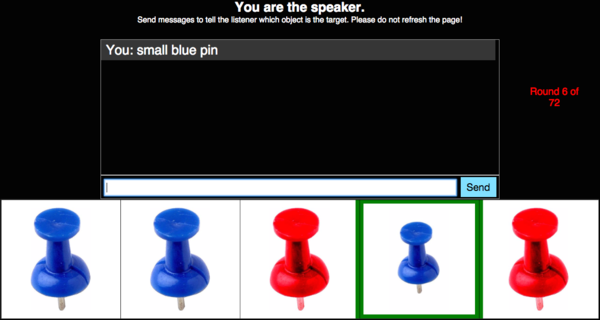
\includegraphics[width=\textwidth]{pics/speaker-perspective-small.png}
\caption{Speakers' perspective}
\label{fig:speakerpersp}
\end{subfigure}

\begin{subfigure}{\textwidth}
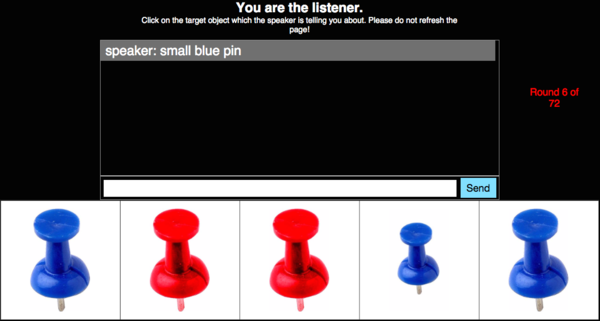
\includegraphics[width=\textwidth]{pics/listener-perspective-small.png}
\caption{Listeners' perspective.}
\label{fig:listenerpersp}
\end{subfigure}
\caption{Example displays from the  (a) speaker's and the  (b)  listener's perspective on a \emph{size-sufficient 4-2} trial.}
\label{fig:speakerlistenerperspective}
\end{figure}

\subsection{Experiment 1: scene variation in modified referring expressions}
\label{sec:exp1-scenevar}

To test the model's predictions, we conducted an interactive web-based written production study within a reference game setting.\footnote{See \appref{app:replication}  for a validation of the general paradigm, in which we qualitatively replicate the findings of \citeA{gatt2011} with a different set of stimuli.} Speakers and listeners were shown arrays of objects of that could vary in color and size. Speakers were asked to produce a referring expression to allow the listener to identify a target object. We manipulated the number of distractor objects in the grid, as well as the variation in color and size among distractor objects.

\subsubsection{Method}


\paragraph{Participants}

We recruited 60 pairs of participants (120 participants total) over Amazon's Mechanical Turk who were each paid \$1.75 for their participation. An additional 38 trials that were contributed by 4 speakers who prematurely dropped out of the experiment and who could therefore not be compensated for their work, were also included. \jd{should we be excluding these? they look like normal trials.} Here and in all other experiments reported in this paper, participants' IP address was limited to US addresses and only participants with a past work approval rate of at least 95\% were accepted. %The data of five pairs were excluded from analysis because one of the participants dropped out before completing the experiment.

\paragraph{Procedure}

Participants were paired up through a real-time multi-player interface \cite{Hawkins15_RealTimeWebExperiments}. For each pair, one participant was assigned the speaker role and one the listener role. They  initially received written instructions that informed participants that one of them would be the Speaker and the other the Listener. They were further told that they would see some number of objects on each round and that the speaker's task is to communicate one of those objects, marked by a green border, to the listener. They were explicitly told that using locative modifiers would be useless because the order of objects on their partner's screen would be different than on their own screen. Before continuing to the experiment, participants were required to correctly answer a series of questions about the experimental procedure. These questions are listed in \appref{app:numdistractors}.

On each trial participants saw an array of objects. The array contained the same objects for both speaker and listener, but the order of objects was randomized and was typically different for speaker and listener. In the speaker's display, one of the objects -- henceforth the \emph{target} -- was highlighted with a green border. See \figref{fig:speakerlistenerperspective} for an example of the listener's and speaker's view on a particular trial.

The speaker produced a referring expression to communicate the target to the listener by typing in a chat window. After pressing Enter or clicking the `Send' button, the speaker's message was shown to the listener. The listener then clicked on the object they thought was the target, given the speaker's message.  Once the listener clicked an object, a red border appeared around that object in both the listener and the speaker's display for 1 second before advancing to the next trial.

Both speakers and listeners could write in the chat window, allowing listeners to request clarification if necessary. Listeners could only click on an object and advance to the next trial once the speaker had sent a message. 


\paragraph{Materials}

Participants proceeded through 72 trials. Of these, half were critical trials of interest and half were filler trials. On critical trials, we varied the feature that was sufficient to mention for uniquely establishing reference, the total number of objects in the array, and  the number of objects that shared the non-sufficient feature with the target. 

Objects varied in color and size. On 18 trials, color was a sufficient property for distinguishing the target. On the other 18 trials, size was sufficient. See \figref{fig:speakerlistenerperspective} for an example of a size-sufficient trial from both the speaker's and the listener's perspective. 

We further varied the amount of variation the scene by varying the number of distractor objects in each array (2, 3, or  4) and the number of distractors that did shared the non-sufficient feature value with the target. That is, when size was the sufficiently distinguishing property, we varied the number of distractors that shared the same color as the target. This number had to be at least one, since otherwise the non-sufficient property would have been sufficient for uniquely establishing reference, i.e.~it would not have been redundant to mention it. Each total number of distractors was crossed with each possible number of distractors that shared the non-sufficient property, leading to the following nine conditions: \emph{2-1, 2-2, 3-1, 3-2, 3-3, 4-1, 4-2, 4-3,} and \emph{4-4}, where the first number indicates the total number and the second number the shared number of distractors. Each condition occurred twice with each sufficient dimension. Objects never differed in type within one array (e.g., all objects are thumbtacks in \figref{fig:speakerlistenerperspective} but always differed in type across trials. Each object type could occur in two different sizes and two different colors. We deliberately chose photo-realistic objects of intuitively fairly typical colors. The 36 different object types and the colors they could occur with are listed in \appref{app:itemtypes}. 


Fillers were target trials from Exp.~2, a replication of \cite{graf2016}. Each filler item contained a three-object grid. None of the filler objects occurred on target trials. Objects stood in various taxonomic relations to each other and required neither size nor color mention for unique reference. See \sectionref{sec:exp2-reflevel} for a description of these materials.

\subsubsection{Data pre-processing and exclusion}

We collected 2138 referential expressions. \jd{Caroline, this number isn't 60*36, which would be 2160 -- is that because there are already some exclusions that went into data/colsizeCor\_manModified.csv? If so, what were they?} Because we did not restrict participants' utterances in any way, they produced many different kinds of expressions to refer to the target. Testing the model's predictions required, for each trial, either excluding it or classifying the produced utterance as an instance of a \emph{color}-only mention, a \emph{size}-only mention, or a \emph{color-and-size} mention. To this end we conducted the following semi-automatic data pre-processing. 

In a first step, an R script automatically checked whether (what the experimenters deemed to be) the target's color or size was included in the utterance. In this way, \red{XXX \%} of cases were classified as containing a size or color term. However, this did not capture that sometimes, a participant produced a different color or size term than the one we had intended (e.g., \emph{pink} instead of \emph{purple} \red{XXX \%} or \emph{large} instead of \emph{big} \red{XXX \%}) or the expression contained a typo (e.g., \emph{pruple} instead of \emph{purple} \red{XXX \%}). In a second step, one of the authors (CG) therefore manually checked the automatic coding: utterances of an unintended color or size were coded as an instance of the intended color or size if they were similar enough in meaning and utterances with typos were corrected.   Most of the time, participants converged on a convention of mentioning simply the target's size and/or color, e.g., \emph{purple} or \emph{big blue}, without even using an article (e.g., \emph{the}) or mentioning the object's type (e.g., \emph{comb}). Articles were omitted in \red{XXX \%} of cases and object types were omitted in \red{XXX \%} of cases. We did not analyze this any further.

Finally, there were 46 cases (2\%) in which the speaker made reference to the distinguishing dimension in an abstract way, e.g.~\emph{different color}, \emph{unique one}, \emph{ripest}, \emph{very girly}, or \emph{guitar closest to viewer}. While interesting as utterance choices,\footnote{Certain participants seemed to have deliberately used this as a strategy even though simply mentioning the distinguishing property would have been shorter in most cases. In all, only 12 participants produced these kinds of utterances: one 18 times, one 8 times, one 6 times, two 3 times, one 2 times, and the remaining six only once each.} these cases were excluded from the analysis. After the exclusion, 2092 cases classified as one of \emph{color}, \emph{size}, or \emph{color-and-size} entered into the analysis.

\jd{Caroline, is there anything else we should mention here?}

\subsubsection{Results}

\jd{Hm, I ended up excluding another 13 cases where speakers mentioned the insufficient dimension -- of these, 6 are true cases of "wrongly" mentioning color instead of size. Another 3 are cases where color is sufficient but speakers say "smallest color","small different color","bigger off a shade", all of which seem nonsensical to me but were categorized as size mentions. The final four are interesting cases of color overmodification where instead of making reference to size, the speaker -- it's only one person -- is making reference to distance ("orange cap closest to  viewer", "brown belt farthest from viewer"). This leaves us with 2079 cases to analyze. Does this seem like the right thing to have done?}

Proportions of redundant \emph{color-and-size} and minimal \emph{color} or \emph{size} utterances are shown in \figref{fig:exp1results} alongside model results (to be explained further in \sectionref{sec:modifiermodeleval}). There are three main questions of interest: first, do we replicate the color/size asymmetry in probability of redundant adjective use? Second, do we replicate the previously established effect of increased redundant color use with increasing scene variation? Third, is there an effect of scene variation on redundant size use and if so, is it smaller compared to that on color use, as is predicted under asymmetric color and size adjective fidelities?

We addressed all of these questions in one fell swoop by conducting a mixed effects logistic regression analysis predicting redundant over minimal adjective use from fixed effects of sufficient property (color vs.~size), scene variation (proportion of distractors that does not share the insufficient property value with the target), and the interaction between the two. The model included the maximal random effects structure that allowed the model to converge: by-speaker and by-item random intercepts as well as by-speaker random slopes for scene variation. 

We observed a main effect of sufficient property such that speakers were more likely to redundantly use color than size adjectives ($\beta = 3.61$, $SE = .23$, $p < .0001$), replicating the much-documented color-size asymmetry. We further observed a main effect of scene variation such that redundant adjective use increased with increasing scene variation ($\beta = 4.11$, $SE = .49$, $p < .0001$). Finally, we also observed a significant interaction between sufficient property and scene variation ($\beta = 3.03$, $SE = .81$, $p < .0002$). Simple effects analysis revealed that the interaction is driven by the scene variation effect being much smaller in the \emph{color-sufficient} condition ($\beta = 2.59$, $SE = .78$, $p < .0009$) than in the \emph{size-sufficient} condition ($\beta = 5.63$, $SE = .45$, $p < .0001$), as predicted under the assumption that size modifiers are noisier than color modifiers.



\begin{figure}
\centering
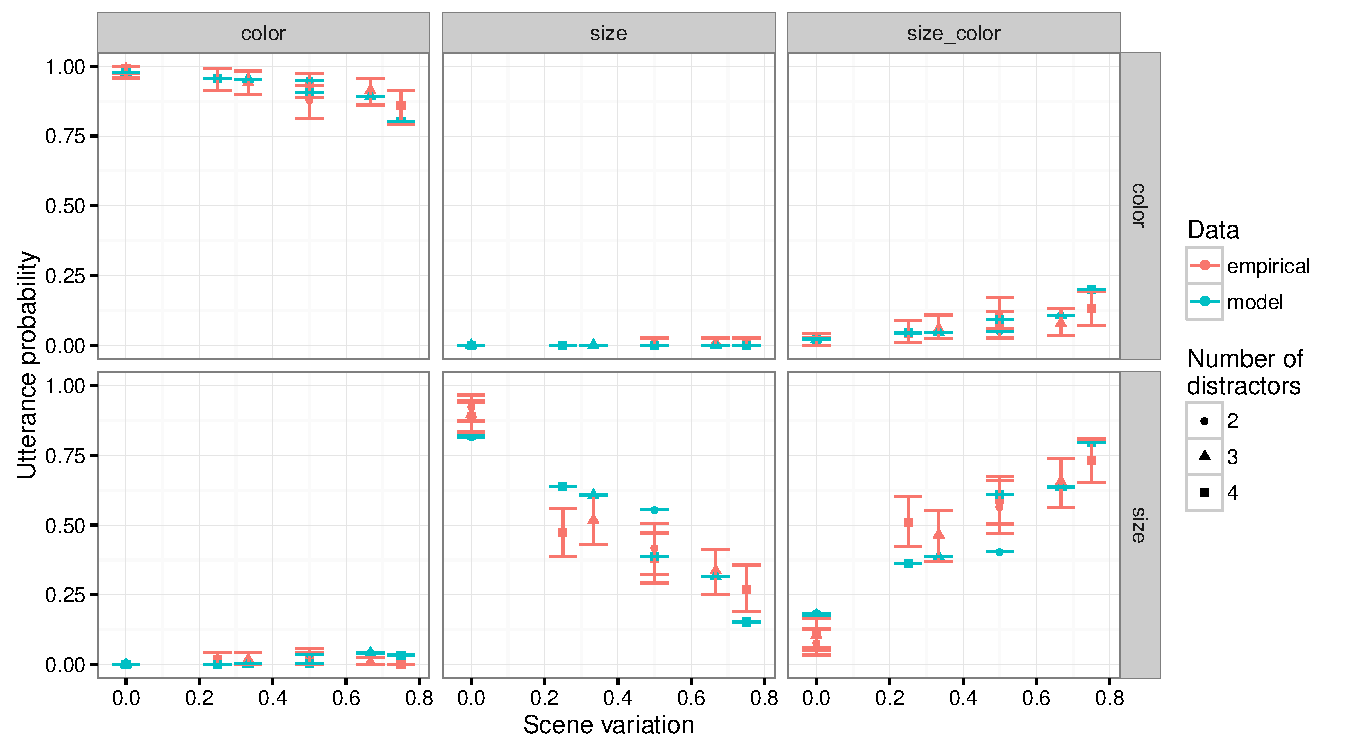
\includegraphics[width=\textwidth]{../../../models/1_basic_overinformativeness/results_bda/graphs/scenevariation-fixed-reducedconditions}
\caption{Empirical utterance proportions  (red)  alongside point-wise maximum a posteriori (MAP) estimates of the model's posterior predictives for utterance probability (blue) as a function of scene variation. Rows indicate the sufficient dimension, columns the produced utterance. Here and in all following plots, error bars indicate 95\% bootstrapped confidence intervals.}
\label{fig:exp1results}
\end{figure}


\subsection{Model evaluation}
\label{sec:modifiermodeleval}

% Extra info: 10000 samples, burn 3000, uniform drift, acceptance rate .4

We performed Bayesian data analysis to generate model predictions and infer likely parameter values, conditioning on the observed production data (coded into \emph{size}, \emph{color}, and \emph{size-and-color} utterances as described above) and integrating over the following free parameters: color fidelity $f_{\textrm{color}}$, size fidelity $f_{\textrm{size}}$, color cost $c_{\textrm{color}}$, size cost $c_{\textrm{size}}$, cost weight $\beta_{\textrm{cost}}$, and speaker rationality parameter $\lambda$. We assumed uniform priors for each parameter: $f_{\textrm{color}} \sim \mathcal{U}(0,1)$, $f_{\textrm{size}} \sim \mathcal{U}(0,1)$, $c_{\textrm{color}} \sim \mathcal{U}(0,2)$, $c_{\textrm{size}} \sim \mathcal{U}(0,2)$, $\beta_{\textrm{cost}} \sim \mathcal{U}(0,5)$, $\lambda  \sim \mathcal{U}(0,12)$.
We implemented both the cognitive and data-analysis models in the probabilistic programming language WebPPL \cite{GoodmanStuhlmuller14_DIPPL}.
Inference for the cognitive model was exact, while we used Markov Chain Monte Carlo (MCMC) to infer posteriors for the six free parameters.

Point-wise maximum a posteriori (MAP) estimates of the model's posterior predictives for each combination of utterance, sufficient dimension, number of distractors, and number of different distractors (collapsing across different items) are compared to empirical data in \figref{fig:modelexp1scatter}. At this level, the model achieves a correlation of $r = .98$. Looking at results additionally on the by-item level yields a correlation of $r = .85$. The model thus does a very good job of capturing the quantitative patterns in the data. This can also be seen in \figref{fig:exp1results}, where model predictions are plotted alongside the empirical proportions by condition. The only clear flaw is that the model predicts greater redundant adjective use than empirically observed when there is no scene variation at all. \jd{a sentence on why}.

\begin{figure}
\centering
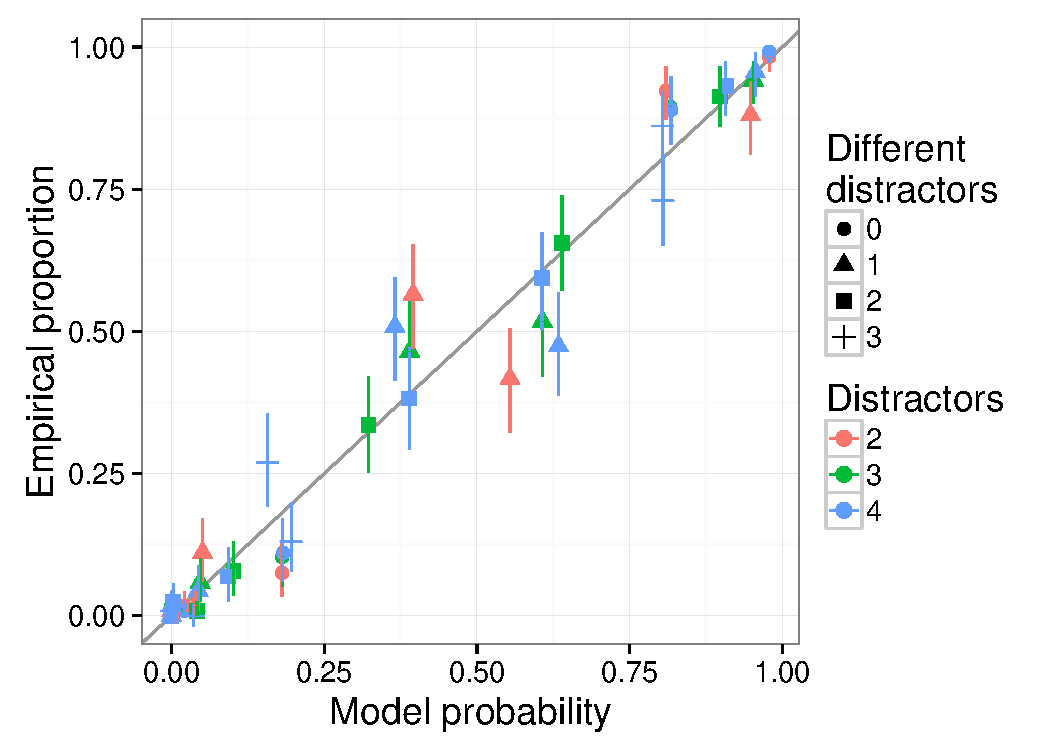
\includegraphics[width=.8\textwidth]{../../../models/1_basic_overinformativeness/results_bda/graphs/predictives-collapsed-fixed-reducedconditions}
\caption{Scatterplot of point-wise maximum a posteriori (MAP) estimates of the model's posterior predictives against empirical proportions ($r=$.99).}
\label{fig:modelexp1scatter}
\end{figure}

Parameter posteriors are shown in \figref{fig:modifierparamposteriors}. Crucially, the fidelity of color is inferred to be higher than that of size -- there is hardly any overlap between the 95\% highest density intervals (HDIs) for the two parameters.\footnote{Analysis of the cases where color fidelity was inferred to be lower than size fidelity reveals that these are also the cases where the cost weight is high -- that is, where the model tries to compensate by increasing the effect of the size-color cost asymmetry (recall that size is always more costly than color). See also \appref{app:fidelity-outliers} for a more detailed analysis.} That is, size modifiers are inferred to be noisier than color modifiers. The relatively high inferred $\lambda$ suggests that this difference in fidelity contributes substantially to the observed color-size asymmetries in redundant adjective use. As for cost, the cost of size modifiers is inferred to be roughly twice that of color, with a non-zero inferred weight on cost. This provides some support for previous claims \red{cite cite} that part of the explanation for the color-size asymmetry stems from the low cognitive cost involved in producing color modifiers compared to size modifiers. However, note that the asymmetry cannot be reduced to cost differences: indeed in \sectionref{sec:} we showed that the color-size asymmetry in redundant adjective use requires an asymmetry in modifier fidelity. An asymmetry in cost only serves to further enhance the asymmetry brought about by the fidelity asymmetry, but cannot carry the redundant use asymmetry on its own.


\begin{figure}
\centering
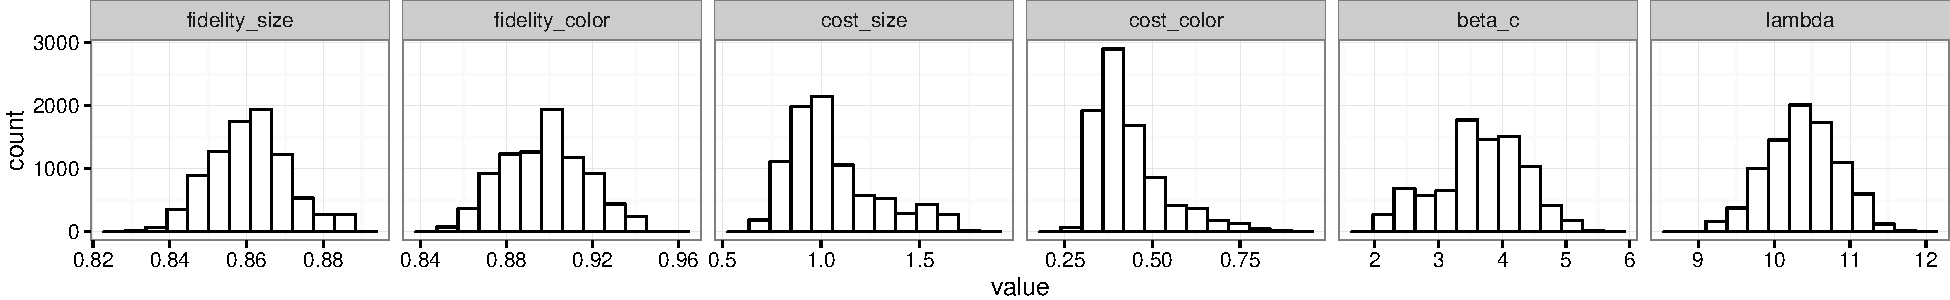
\includegraphics[width=\textwidth]{../../../models/1_basic_overinformativeness/results_bda/graphs/parameterposteriors-fixed-reducedconditions}
\caption{Posterior distribution over model parameters. Maximum a posteriori (MAP)  $f_{\textrm{size}}$ = 0.86, 95\% highest density interval (HDI) = [0.84,0.88]; MAP $f_{\textrm{color}}$ = 0.90, HDI = [0.85,0.93]; MAP $c_{\textrm{size}}$ = .91, HDI = [.75, 1.9]; MAP $c_{\textrm{color}}$ = 0.36, HDI = [0.31,0.85]; MAP $\beta_c$ = 2.2, HDI = [1.7,4.6]; MAP $\lambda$ = 10.5, HDI = [9.6,11.3]}
\label{fig:modifierparamposteriors}
\end{figure}




\subsection{Modeling speakers' choice of reference level}
\label{sec:reflevelmodel}

\jd{motivation, bridge: ref level selection as analogous to property selection -- both fall under what kees et al call "content selection"}

This is the innovation: rather than assuming that words have deterministic truth conditions, we assign each word a graded meaning. For instance, the word ``dog'' describes a dalmatian better than a grizzly bear, but it also describes a grizzly bear better than a tennis ball.
The speaker also seeks to be parsimonious: the speaker utility includes both informativeness and word cost; cost includes both a word's length and its frequency.

Formally, we start by specifying a literal listener $L_0$ who hears a word $w$ at a particular level of reference  in the context of some set of objects $\mathcal{O}$ and forms a distribution over the referenced object, $o \in \mathcal{O}$ : 
$$P_{L_0}(o | w) \propto \denote{w}(o).$$
Here $\denote{w}(o)$ is the lexical meaning of the word $w$ when applied to object $o$. We take this to be a real number indicating the degree of acceptability of object $o$ for category $w$. 

We relate this to our empirically elicited typicality norms \jd{first introduce typicality norms!} via an exponential relationship: $\denote{w}(o)=\exp(\text{typicality}(o,w))$.\footnote{Cases where typicality was not elicited were assumed to have typicality $0$.}
This relationship is motivated by considering the effect of a small difference in typicality on choice probability: in our elicitation experiment a small difference in rating should mean the same thing at the top and bottom of the scale (it is visually equivalent on the slider that participants used).
In order for a small difference in typicality rating to have a constant effect on relative choice probability (which is a ratio), the relationship must be exponential. 

Next, we specify a speaker $S_1$ who intends to refer to a particular object $o \in \mathcal{O}$ and chooses among possible words $w \in {\mathcal W}(o)$.
We take ${\mathcal W}(o)$ to be the three words for $o$ at the sub, basic, and super level.
The speaker chooses among these nouns in a way that is influenced by informativeness of the noun for the literal listener ($\ln P_{L_0}(o | w)$), the frequency ($\hat{c}_f$) and the length  ($\hat{c}_l$), each weighted by a free parameter:
$$P_{S_1}(w | o) \propto \exp(\lambda \ln P_{L_0}(o | w) + \beta_f \hat{c}_f  + \beta_l \hat{c}_l)$$
Length cost $\hat{c}_l$ was defined as the empirical mean number of characters used to refer at that level and frequency cost $\hat{c}_f$ was the log frequency in the Google Books corpus from 1960 to the present. 

\jd{put this last paragraph somewhere else?}
We performed Bayesian data analysis to generate model predictions, conditioning on the observed production data (coded into sub, basic, and super level descriptions as described above) and integrating over the three free parameters.
We assumed uniform priors for each parameter: $\lambda  \sim Unif(0,20)$, $\beta_f \sim Unif(0,5)$, $\beta_l \sim Unif(0,5)$.
We implemented both the cognitive and data-analysis models in the probabilistic programming language WebPPL \cite{GoodmanStuhlmuller14_DIPPL}.
Inference for the cognitive model was exact, while we used Markov Chain Monte Carlo (MCMC) to infer posteriors for the three free parameters.

\jd{insert qualitative plots and describe -- a) model predictions for the 4 different contexts if no cost diffs and no typicality; b) model predictions for the 4 different contexts when competitor is costlier/less costly but no typicality; c) model predictions for the 4 different contexts when competitor typicality is greater/lesser but no cost diffs; d) combine both or too complex? -- CAROLINE NEEDS TO FINISH MODEL EXPLORATION FOR US TO BE ABLE TO DO THIS}

\subsection{Experiment 2: choice of reference level}
\label{sec:exp2-reflevel}


\section{Typicality effects}
\label{sec:typicality}

\jd{extension of basic modifiers model to color typicality effects. Show qualitative result. Then discuss empirically elicited typicality norms for colro and simplay type expression in exp.~1 and show that typicality matters and that we find a typicality effect in our data empirically? Maybe already discuss the issue of compositionality here instead of in the GD.}

\section{General Discussion}
\label{sec:gd}

\begin{itemize}
	\item talk about how the approach applies to other referring expressions like those mentioned in the intro (indefinite, post-nominal modification pronouns)
	\item nature of numbers in non-deterministic semantics (we see that typicality effects fall out of treating the numbers in the semantics as typicality values for noun choice, and the same if we make up values for modifier choice -- but how do we get here compositionally? one would ideally model the structure in the prior (rich world knowledge), ie the statistical correlations between different dimensions (type -- banana, color -- blue/yellow, etc) and have the fidelity/noise values emerge from THAT compositionally!
	\item talk about how our approach fits in with incremental stories of overspecification?
	\item The work reported here clearly shows that overmodified referring expressions, contrary to some claims in the literature \cite{Engelhardt2011} \red{who say overmodification ipmairs comprehension}, contribute more utility than `minimally' specified referring expressions.
\end{itemize}
%
\red{There's a parallel to be made between typicality effects on ``overmodification" and the literature on instrument mention. For example, \cite{brown1987} showed that atypical instruments are more likely to be mentioned than typical ones ("The man was stabbed with an ice pick", not "The man was stabbed with a knife"). Their account of the effect is that speakers do this for speaker-internal reasons. \cite{lockridge2002} replicated the original finding in a story retelling scenario, but also manipulated whether or not the addressees saw pictures of the actions. Without pictures, there were even more mentions of atypical objects, which they take as evidence that the typicality effect is an audience design effect. THIS IS COOL AND PICKS UP ON THE SPEAKER-OR-LISTENER POINT YOU RAISE IN THE INTRO IN THE TYPICALITY PART!!!!!}
%
\appendix

\section{Validation of interactive web-based written production paradigm}
\label{app:replication}

\red{make sure to discuss why overall we have lower overspecification rates -- probably because of color typicality!! we had pretty typical colors in our stimuli}

\section{Pre-experiment quiz}
\label{app:numdistractors}

Before continuing to the main experiment, each participant had to correctly respond ``True'' or ``False'' to the following statements. Correct answers are given in parentheses after the statement.

\begin{itemize}
	\item The speaker can click on an object. (False)
	\item The listener wants to click on the object that the speaker is
  telling them about. (True)
  \item  The target is the object which has the red circle around it. (False)
  \item Only the speaker can send messages. (False)
  \item There are a total of 72 rounds. (True)
  \item The locations of the three objects are the same for the speaker and the listener. (False)
\end{itemize}


\section{Item types}
\label{app:itemtypes}

The following table lists all 36 object types from Exp.~\red{XXX} and the colors they appeared in:

\begin{tabular}{l l l l}
\toprule
Object & Colors & Object & Colors \\
\midrule
avocado & black, green & balloon & pink, yellow \\
belt & black, brown & bike & purple, red\\
billiard ball & orange, purple & binder & blue, green \\
book & black, blue & bracelet & green, purple \\
bucket & pink, red & butterfly & blue, purple\\
candle & blue, red & cap & blue, orange \\
chair & green, red & coat hanger & orange, purple \\
comb & black, blue & cushion & blue, orange\\
flower & purple, red & frame & green, pink \\
golf ball & blue, pink & guitar & blue, green\\
hair dryer & pink, purple & jacket & brown, green\\
napkin & orange, yellow & ornament & blue, purple\\
pepper & green, red & phone & pink, white\\
rock & green, purple & rug & blue, purple \\
shoe & white, yellow & stapler & purple, red\\
thumb tack & blue, red & tea cup & pink, white \\
toothbrush & blue, red & turtle & black, brown \\
wedding cake & pink, white & yarn & purple, red\\
\bottomrule
\end{tabular}

\section{Analysis of cases with higher inferred size than color typicality}
\label{app:fidelity-outliers}

\figref{fig:fidelity-outliers-reducedconditions} visualizes all 10,000 samples' from the BDA run on the data from Exp.~1 with an eye towards understanding the cases in which inferred size fidelity was greater than color fidelity. In general, these cases were very unlikely, with a posterior probability of .048. Conditioning on these cases, the probability of a low cost weight was only .23 (only .01 probability overall). That is, where color fidelity was lower than size fidelity, the model tried to achieve the empirical color-size asymmetry by placing greater weight on cost differences, where size was always inferred to be costlier than color.

\begin{figure}
\centering
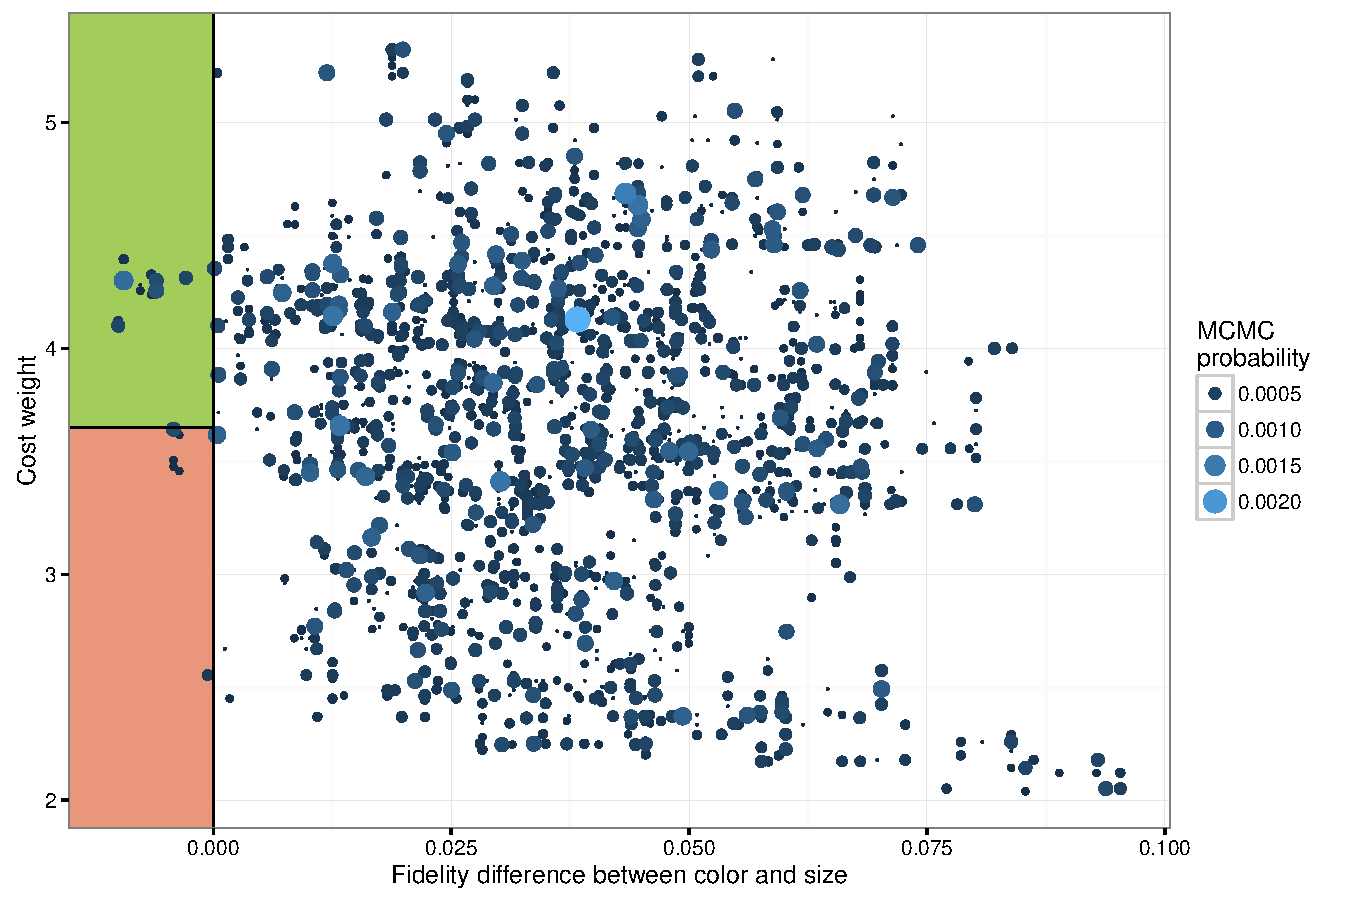
\includegraphics[width=.7\textwidth]{../../../models/1_basic_overinformativeness/results_bda/graphs/fidelity-outliers-fixed-reducedconditions}
\caption{Each sample's cost weight $\beta_c$ against difference between color and size fidelity ($f_{\textrm{color}} - f_{\textrm{size}}$). Green region includes cases with higher inferred size than color fidelity that have a cost weight greater than or equal to the median cost weight. Red region includes cases with higher inferred size than color fidelity that have a cost weight lower than the median cost weight. Dot size and color indicates parameter values' posterior probability.}
\label{fig:fidelity-outliers-reducedconditions}
\end{figure}



\section{Gatt replication}
\red{report Gatt et al 2011 replication}

\bibliographystyle{apacite}

\setlength{\bibleftmargin}{.125in}
\setlength{\bibindent}{-\bibleftmargin}

\bibliography{bibs}


\end{document}
